\documentclass{standalone}
\usepackage{tikz}
\usepackage{calc}
\usepackage{pgffor}
\usetikzlibrary{patterns}
\begin{document}
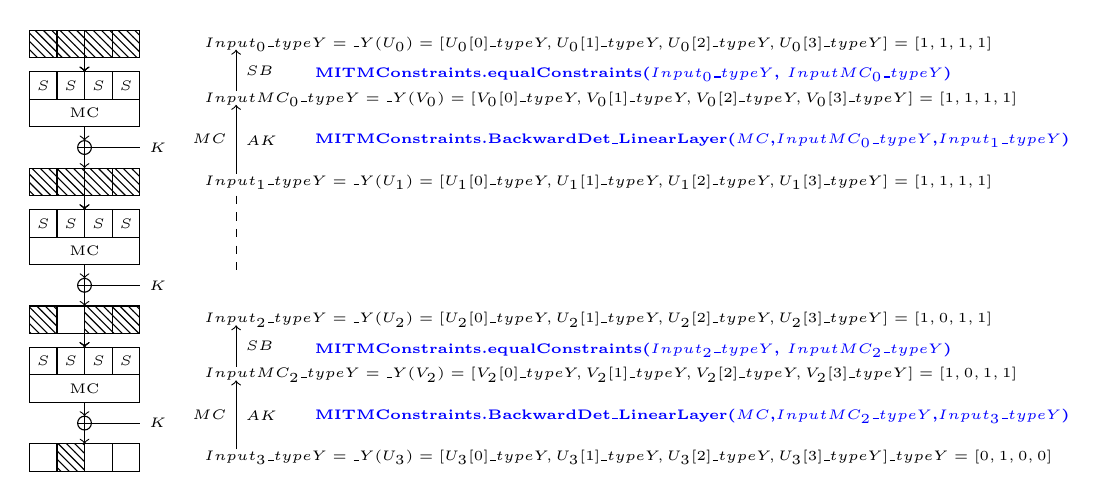
\begin{tikzpicture}[scale=0.35]
%\begin{scope}[yshift = -5cm]
%\fill[red](0,0) rectangle+(1,1);
%\fill[red](1,0) rectangle+(1,1);
%\fill[red](2,0) rectangle+(1,1);
%\end{scope}
%\begin{scope}[yshift = -10cm]
%\fill[red](0,0) rectangle+(1,1);
%\fill[red](2,0) rectangle+(1,1);
%\fill[red](3,0) rectangle+(1,1);
%\end{scope}
\begin{scope}[yshift = 0cm]
\draw[pattern = north west lines](0,0) rectangle+(1,1);
\draw[pattern = north west lines](1,0) rectangle+(1,1);
\draw[pattern = north west lines](2,0) rectangle+(1,1);
\draw[pattern = north west lines](3,0) rectangle+(1,1);
%\draw[pattern = north east lines](3,0) rectangle+(1,1);

\end{scope}
\begin{scope}[yshift = -5cm]
%\draw[pattern = north east lines](0,0) rectangle+(1,1);
%\draw[pattern = north east lines](1,0) rectangle+(1,1);
%\draw[pattern = north east lines](2,0) rectangle+(1,1);

\draw[pattern = north west lines](2,0) rectangle+(1,1);
\draw[pattern = north west lines](3,0) rectangle+(1,1);
\draw[pattern = north west lines](0,0) rectangle+(1,1);
\draw[pattern = north west lines](1,0) rectangle+(1,1);
\end{scope}
\begin{scope}[yshift = -10cm]
%\draw[pattern = north east lines](0,0) rectangle+(1,1);
%\draw[pattern = north east lines](1,0) rectangle+(1,1);
%\draw[pattern = north east lines](2,0) rectangle+(1,1);
%\draw[pattern = north east lines](3,0) rectangle+(1,1);
\draw[pattern = north west lines](3,0) rectangle+(1,1);
\draw[pattern = north west lines](0,0) rectangle+(1,1);
\draw[pattern = north west lines](2,0) rectangle+(1,1);
\end{scope}
\begin{scope}[yshift = -15cm]
%\draw[pattern = north east lines](0,0) rectangle+(1,1);
%\draw[pattern = north east lines](1,0) rectangle+(1,1);
%\draw[pattern = north east lines](2,0) rectangle+(1,1);
%\draw[pattern = north east lines](3,0) rectangle+(1,1);

\draw[pattern = north west lines](1,0) rectangle+(1,1);
\end{scope}
\foreach \z in {0,1,2}{
\begin{scope}[yshift = -\z* 5 cm]
\draw (0,0) grid +(4,1);
\foreach \y in {0,1,2,3}{\draw[->](2,0)--+(0,-0.5);
\draw(\y,-1.5) rectangle node{\tiny{$S$}} +(1,1);
}
\draw (0,-2.5) rectangle node{\tiny{MC}} +(4,1);
\draw[->] (2,-2.5)--+(0,-0.5);
\draw (1.75,-3.25)--+(0.5,0);
\draw (2,-3.25) circle (0.25);
\draw (4,-3.25) --(2.25,-3.25);
\node[right] at (4,-3.25) {\tiny{$K$}};
\draw[->](2,-3)--+(0,-1);
\end{scope}}

\begin{scope}[yshift = -15 cm]
\draw (0,0) grid +(4,1);
\end{scope}


\begin{scope}[yshift = 0 cm, xshift = 6 cm]
\node[right] at (0, 0.5) {\tiny{$Input_0\_typeY = \_Y(U_0) = [U_0[0]\_typeY,U_0[1]\_typeY,U_0[2]\_typeY,U_0[3]\_typeY]=[1,1,1,1]$}};

\draw[->] (1.5, -1.2)-- node[right] {\tiny{$SB$}} +(0,1.5);
\node[right] at (4, -0.6) {\textbf{\textcolor{blue}{\tiny{MITMConstraints.equalConstraints($Input_0\_typeY$, $InputMC_0\_typeY$)}}}};

\node[right] at (0,-1.5) {\tiny{$InputMC_0\_typeY = \_Y(V_0) = [V_0[0]\_typeY,V_0[1]\_typeY,V_0[2]\_typeY,V_0[3]\_typeY]=[1,1,1,1]$}};

\draw[->] (1.5, -4.2)-- node[left] {\tiny{$MC$}} +(0,2.5);
\node[right] at (1.5,-3) {\tiny{$AK$}};
\node[right] at (4, -3) {\textbf{\textcolor{blue}{\tiny{MITMConstraints.BackwardDet\_LinearLayer($MC$,$InputMC_0\_typeY$,$Input_1\_typeY$)}}}};

\node[right] at (0,-4.5) {\tiny{$Input_1\_typeY = \_Y(U_1) = [U_1[0]\_typeY,U_1[1]\_typeY,U_1[2]\_typeY,U_1[3]\_typeY]=[1,1,1,1]$}};

\end{scope}

\draw[dashed](7.5,-5) -- +(0,-3);

\begin{scope}[yshift = -10 cm, xshift = 6 cm]
\node[right] at (0, 0.5) {\tiny{$Input_2\_typeY = \_Y(U_2) = [U_2[0]\_typeY,U_2[1]\_typeY,U_2[2]\_typeY,U_2[3]\_typeY]=[1,0,1,1]$}};

\draw[->] (1.5, -1.2)-- node[right] {\tiny{$SB$}} +(0,1.5);
\node[right] at (4, -0.6) {\textbf{\textcolor{blue}{\tiny{MITMConstraints.equalConstraints($Input_2\_typeY$, $InputMC_2\_typeY$)}}}};

\node[right] at (0,-1.5) {\tiny{$InputMC_2\_typeY = \_Y(V_2) = [V_2[0]\_typeY,V_2[1]\_typeY,V_2[2]\_typeY,V_2[3]\_typeY]=[1,0,1,1]$}};

\draw[->] (1.5, -4.2)-- node[left] {\tiny{$MC$}} +(0,2.5);
\node[right] at (1.5,-3) {\tiny{$AK$}};
\node[right] at (4, -3) {\textbf{\textcolor{blue}{\tiny{MITMConstraints.BackwardDet\_LinearLayer($MC$,$InputMC_2\_typeY$,$Input_3\_typeY$)}}}};

\node[right] at (0,-4.5) {\tiny{$Input_3\_typeY = \_Y(U_3) = [U_3[0]\_typeY,U_3[1]\_typeY,U_3[2]\_typeY,U_3[3]\_typeY]\_typeY=[0,1,0,0]$}};

\end{scope}
\end{tikzpicture}
\end{document}